% !TeX root = ../main.tex
\chapter{Unidad 7: Características subjetivas de la percepción auditiva (Psicoacústica)}
\section*{Objetivo pedagógico}
\noindent\textbf{Objetivo.} Explorar los atributos subjetivos del sonido (sonoridad, altura, timbre, localización, inteligibilidad), entender fenómenos como el enmascaramiento y el efecto de precedencia (Haas), y aplicar estos principios psicofísicos a la práctica fonoaudiológica, como el diseño de audífonos y la evaluación de la audición. Se incluyen ejemplos clínicos, actividades prácticas, recursos multimedia y ejercicios de autoevaluación.

\noindent\textbf{Pregunta inicial.} ¿Por qué un susurro suena más débil que un grito, aunque tengan la misma frecuencia? ¿Cómo localizamos un sonido en una sala ruidosa? ¡Esta unidad te ayudará a entender cómo percibimos el sonido!

\section{Sonoridad e igual sonoridad}

\subsection{Curvas isofónicas ISO 226 (2003)}
Las curvas isofónicas muestran cómo diferentes frecuencias y niveles de presión sonora (dBSPL) producen la misma \textbf{sonoridad} (en fones). A 1 kHz, 1 fon = 1 dBSPL. A niveles bajos ($<$40 fones), el oído es menos sensible a frecuencias graves ($<$250 Hz) y muy agudas ($>$8 kHz).

\begin{quote}
    \textbf{Ejemplo clínico.} En una audiometría, un tono de 125 Hz a 40 dBSPL se percibe más débil que uno de 1 kHz a 40 dBSPL, debido a la menor sensibilidad del oído a bajas frecuencias.
\end{quote}


\begin{figure}[h]
    \centering
    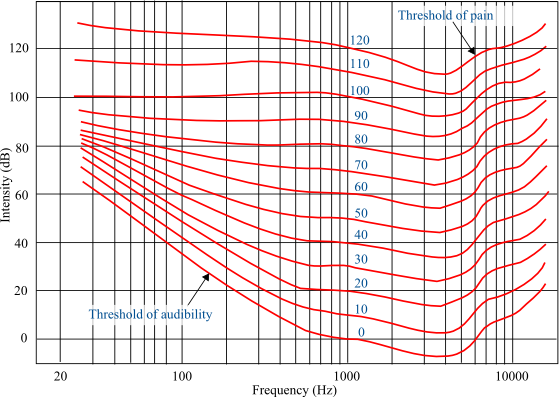
\includegraphics[width=0.9\textwidth]{figures/FletcherMunson.png}
    \caption{Curvas isofónicas de Fletcher y Munson.}
    \label{fig:isofonicas}
\end{figure}



\subsection{Ley de Stevens y conversión a sones}
La escala de \textbf{sones} mide la sonoridad de forma lineal:
\[
\text{sones} = 2^{\frac{\text{fones} - 40}{10}}.
\]
Por ejemplo, 70 fones = $2^{(70-40)/10} = 8$ sones, percibido como 8 veces más intenso que 40 fones (1 son).

\begin{quote}
    \textbf{Ejemplo clínico.} Al ajustar un audífono, aumentar de 70 dBSPL (8 sones) a 80 dBSPL (16 sones) a 1 kHz duplica la sonoridad, pero puede causar molestias si no se calibra cuidadosamente.
\end{quote}

\textbf{Actividad práctica.} Usa Tone Generator (gratis en línea) para comparar un tono de 1 kHz a 40 dB con uno de 125 Hz a 40 dB. Nota cómo el tono grave se percibe más débil, reflejando las curvas isofónicas.

\section{Umbrales y resonancia del CAE}
El \textbf{umbral absoluto} de audición es aproximadamente 0 dBSPL a 1 kHz en un campo libre (sin reflexiones). El canal auditivo externo (CAE) amplifica frecuencias de 2–4 kHz en 10–15 dB debido a su resonancia ($\approx$3.4 kHz), haciendo el oído más sensible en este rango.

\begin{quote}
    \textbf{Ejemplo clínico.} En una cabina audiométrica, el ruido de fondo debe ser $<$35 dBA para no enmascarar los umbrales de audición, especialmente en frecuencias altas donde el oído es más sensible.
\end{quote}

\section{Atributos subjetivos principales}
El sonido se percibe a través de varios atributos:
\begin{description}
    \item[\textbf{Altura (pitch):}] Depende de la frecuencia fundamental ($f_0$). Por ejemplo, 120 Hz suena grave (voz masculina), 250 Hz más agudo (voz femenina). El \textbf{pitch residual} ocurre cuando el cerebro reconstruye $f_0$ aunque esté ausente.
    \item[\textbf{Timbre:}] Determinado por los armónicos y su evolución. Diferencia un violín de una flauta, o la voz de un paciente con disfonía.
    \item[\textbf{Sonoridad:}] Relacionada con la amplitud y el ancho de banda. Un ruido amplio (como el viento) suena más fuerte que un tono puro al mismo nivel dB.
    \item[\textbf{Duración subjetiva:}] Sonidos $<$200 ms parecen más cortos; el umbral temporal es $\approx$10 ms, afectando la percepción de consonantes rápidas.
\end{description}

\begin{quote}
    \textbf{Ejemplo clínico.} En la rehabilitación de pacientes con audífonos, ajustar el timbre (amplificando armónicos) mejora la claridad del habla, mientras que la sonoridad debe equilibrarse para evitar el reclutamiento.
\end{quote}

\section{Enmascaramiento y banda crítica}

\subsection{Concepto}
El \textbf{enmascaramiento} ocurre cuando un sonido (masker) eleva el umbral de detección de otro (signal). La \textbf{banda crítica} (ERB, Equivalent Rectangular Bandwidth) es el rango de frecuencias donde la energía se suma:
\[
\text{ERB} = 24.7 (4.37 f + 1) \, \text{Hz},
\]
donde $f$ está en kHz. Por ejemplo, a 1 kHz, ERB $\approx$ 108 Hz.

\begin{quote}
    \textbf{Ejemplo clínico.} En audiometría, se usa ruido de banda estrecha para enmascarar el oído contralateral, asegurando que solo el oído evaluado detecte el tono puro.
\end{quote}


\begin{figure}[h]
    \centering
    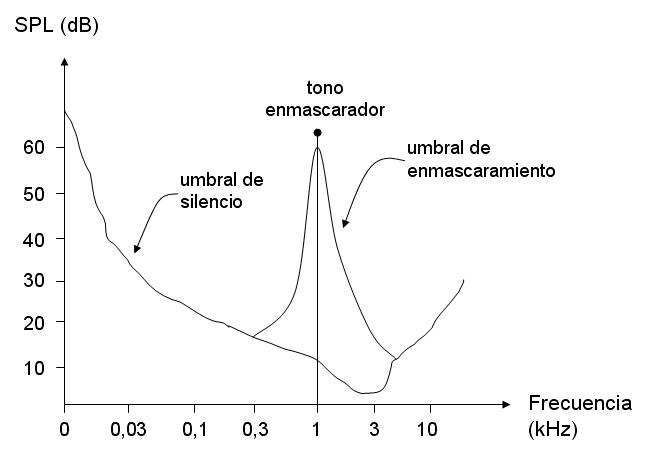
\includegraphics[width=0.9\textwidth]{figures/enmascaramiento.png}
    \caption{Umbral de enmascaramiento dado por un tono puro.}
\end{figure}


\textbf{Actividad práctica.} Usa Tone Generator para reproducir un tono de 1 kHz a 60 dB y otro de 1.1 kHz a 20 dB simultáneamente. Nota cómo el tono más fuerte (masker) dificulta escuchar el más débil (signal).

\section{Sonidos impulsivos e inteligibilidad}

\subsection{Sensibilidad temporal}
Sonidos breves ($<$50 ms), como consonantes (5–15 ms), requieren 10–15 dB más para percibirse con igual sonoridad que sonidos largos. En salas reverberantes, los ecos dificultan la percepción de estas consonantes.

\subsection{Índice de inteligibilidad}
La \textbf{inteligibilidad del habla} (IL\%) depende de la relación señal-ruido (SNR) y el tiempo de reverberación ($T_{60}$):
\[
\text{IL\%} \approx 100 \frac{\text{SNR} - \text{SNR}_{50}}{30}, \quad \text{SNR}_{50} \approx 2 \, \text{dB}.
\]
Por ejemplo, una SNR de 12 dB da $\approx$67\% de inteligibilidad.

\begin{quote}
    \textbf{Ejemplo clínico.} En un aula con reverberación alta ($T_{60}$ $>$ 1 s), los niños con hipoacusia tienen dificultad para entender palabras debido a la baja inteligibilidad.
\end{quote}

\section{Efecto de precedencia (Haas)}
El cerebro fusiona un sonido directo con sus reflexiones si llegan dentro de $<$50 ms, mejorando la sonoridad sin afectar la localización. Retardos de 15–20 ms son ideales en sistemas de refuerzo sonoro (como altavoces en auditorios).

\begin{quote}
    \textbf{Ejemplo clínico.} En una sala de conferencias, los altavoces deben retrasarse $<$20 ms respecto a la voz del orador para que los pacientes con audífonos perciban un sonido claro y localizado.
\end{quote}

\section{Localización binaural}

\subsection{Pistas físicas}
El cerebro usa dos pistas principales para localizar sonidos:
\begin{itemize}
    \item \textbf{Diferencia interaural de tiempo (DIT):} Retardo entre oídos (máximo $\approx$0.69 ms), efectivo para frecuencias $<$1.5 kHz.
    \item \textbf{Diferencia interaural de intensidad (DII):} Atenuación por la sombra de la cabeza (hasta 20 dB a 6 kHz).
\end{itemize}

\subsection{Pistas espectrales monaurales}
La forma del pabellón altera el espectro del sonido, ayudando a detectar la altura (arriba/abajo).

\begin{quote}
    \textbf{Ejemplo clínico.} Un audífono direccional usa DIT y DII para mejorar la localización en entornos ruidosos, ayudando al paciente a enfocarse en una conversación.
\end{quote}

\begin{figure}[h]
    \centering
    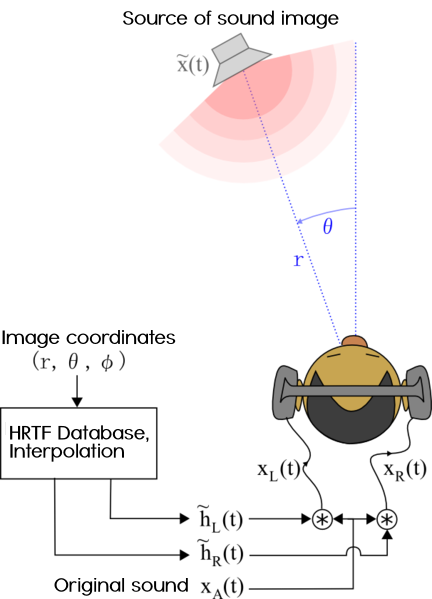
\includegraphics[width=0.5\textwidth]{figures/localizacion_fuentes.png}
    \caption{Sistema de localización binaural.}
    \label{localizacion_fuentes}
\end{figure}

\section{Efecto cocktail party}
El cerebro agrupa sonidos por similitud espectral y espacial, permitiendo enfocarse en una voz en un entorno ruidoso (como una fiesta). Los audífonos direccionales mejoran la SNR física ($\approx$6 dB), potenciando esta capacidad.

\begin{quote}
    \textbf{Ejemplo clínico.} Un paciente con audífonos direccionales puede seguir una conversación en un restaurante al reducir el ruido de fondo, aprovechando el efecto cocktail party.
\end{quote}

\textbf{Actividad práctica.} En un lugar ruidoso (como un café), intenta seguir una conversación cercana mientras escuchas ruido de fondo. Nota cómo tu cerebro “filtra” la voz objetivo, simulando el efecto cocktail party.

\section{Ejemplos prácticos}
\begin{enumerate}
    \item \textbf{Conversión a sones.} 60 fones = $2^{(60-40)/10} = 4$ sones.
    \item \textbf{Enmascaramiento.} Un masker de 60 dBSPL eleva el umbral de 20 dBSPL a $\approx$ 60 dBSPL, ya que la banda crítica integra la energía del masker.
    \item \textbf{DII.} Un tono de 6 kHz a 90° (sombra de cabeza) tiene una DII de $\approx$ 20 dB, haciendo que el sonido sea mucho más débil en el oído opuesto.
\end{enumerate}

\section{Ejercicios de autoevaluación}

\begin{enumerate}

    \item Explica por qué un ventilador que genera una señal de 31.5 Hz muestra una lectura menor en dBA que en dBZ. Usa la tabla de ponderaciones de la Unidad 5.
    \item Diseña un protocolo de enmascaramiento para una audiometría ósea a 1 kHz, considerando la banda crítica.
    \item Justifica por qué un sistema de refuerzo sonoro en una sala debe usar retardos $<$20 ms para mantener la localización.
    \item Usa Tone Generator para comparar un tono de 1 kHz a 60 dB con uno de 250 Hz a 60 dB. Explica la diferencia en sonoridad.
    
\end{enumerate}

\section{Recursos recomendados}

\begin{itemize}

    \item Video: \href{https://www.youtube.com/watch?v=csQkSZX9aJw&ab_channel=SrinathSrinivasan}{``Equal Loudness Contour explained''}. 
    \item App: Tone Generator (gratis). Prueba tonos y enmascaramiento.
    \item App: Audacity (gratis). Analiza espectros y timbres.
    \item Libro: B. C. J. Moore, \emph{An Introduction to the Psychology of Hearing}, capítulos 5–8.
    
\end{itemize}

\section*{Glosario}
\begin{description}
    \item[\textbf{Fon:}] Unidad de sonoridad, igual a dBSPL a 1 kHz.
    \item[\textbf{Son:}] Escala lineal de sonoridad (1 son = 40 fones).
    \item[\textbf{Banda crítica:}] Rango de frecuencias donde la energía se suma, afecta el enmascaramiento.
    \item[\textbf{DIT/DII:}] Diferencias interaurales de tiempo e intensidad, para localización.
    \item[\textbf{Efecto cocktail party:}] Capacidad de enfocar un sonido en un entorno ruidoso.
\end{description}

\section*{Resumen}
\begin{itemize}
    \item \textbf{Sonoridad:} Depende de la frecuencia y nivel (curvas isofónicas); se mide en fones y sones.
    \item \textbf{Atributos:} Altura (frecuencia), timbre (armónicos), duración (temporal).
    \item \textbf{Enmascaramiento:} Un sonido fuerte eleva el umbral de otro, clave en audiometrías.
    \item \textbf{Localización:} Usa DIT, DII y pistas monaurales; mejora con audífonos direccionales.
\end{itemize}

\bigskip
\noindent\emph{Conclusión.} La psicoacústica explica cómo percibimos el sonido más allá de su física, guiando el diseño de audífonos, pruebas audiométricas y entornos acústicos. Comprender la sonoridad, el enmascaramiento y la localización mejora la rehabilitación auditiva y la calidad de vida de los pacientes.



%%%%%%%%%%%%%%%%%%%%%%%%%%%%%%%%%%%%%%%%%%%%%%%%%%%%%%%%%%%%%%%%%%%%%%%%%%%%%%%%%%%%%%%%%%%%%%%%%%
